\documentclass[journal]{vgtc}                % final (journal style)
%\documentclass[review,journal]{vgtc}         % review (journal style)
%\documentclass[widereview]{vgtc}             % wide-spaced review
%\documentclass[preprint,journal]{vgtc}       % preprint (journal style)

%% Uncomment one of the lines above depending on where your paper is
%% in the conference process. ``review'' and ``widereview'' are for review
%% submission, ``preprint'' is for pre-publication, and the final version
%% doesn't use a specific qualifier.

%% Please use one of the ``review'' options in combination with the
%% assigned online id (see below) ONLY if your paper uses a double blind
%% review process. Some conferences, like IEEE Vis and InfoVis, have NOT
%% in the past.

%% Please note that the use of figures other than the optional teaser is not permitted on the first page
%% of the journal version.  Figures should begin on the second page and be
%% in CMYK or Grey scale format, otherwise, colour shifting may occur
%% during the printing process.  Papers submitted with figures other than the optional teaser on the
%% first page will be refused. Also, the teaser figure should only have the
%% width of the abstract as the template enforces it.

%% These few lines make a distinction between latex and pdflatex calls and they
%% bring in essential packages for graphics and font handling.
%% Note that due to the \DeclareGraphicsExtensions{} call it is no longer necessary
%% to provide the the path and extension of a graphics file:
%% 
\includegraphics{diamondrule} is completely sufficient.
%%
\ifpdf%                                % if we use pdflatex
  \pdfoutput=1\relax                   % create PDFs from pdfLaTeX
  \pdfcompresslevel=9                  % PDF Compression
  \pdfoptionpdfminorversion=7          % create PDF 1.7
  \ExecuteOptions{pdftex}
  \usepackage{graphicx}                % allow us to embed graphics files
  \DeclareGraphicsExtensions{.pdf,.png,.jpg,.jpeg} % for pdflatex we expect .pdf, .png, or .jpg files
\else%                                 % else we use pure latex
  \ExecuteOptions{dvips}
  \usepackage{graphicx}                % allow us to embed graphics files
  \DeclareGraphicsExtensions{.eps}     % for pure latex we expect eps files
\fi%

%% it is recomended to use ``\autoref{sec:bla}'' instead of ``Fig.~\ref{sec:bla}''
\graphicspath{{figures/}{pictures/}{images/}{./}} % where to search for the images

\usepackage{comment}
\usepackage{microtype}                 % use micro-typography (slightly more compact, better to read)
\PassOptionsToPackage{warn}{textcomp}  % to address font issues with \textrightarrow
\usepackage{textcomp}                  % use better special symbols
\usepackage{mathptmx}                  % use matching math font
\usepackage{times}                     % we use Times as the main font
\renewcommand*\ttdefault{txtt}         % a nicer typewriter font
\usepackage{cite}                      % needed to automatically sort the references
\usepackage{tabu}                      % only used for the table example
\usepackage{booktabs}                  % only used for the table example
\usepackage[]{algorithm2e}

\usepackage[usenames, dvipsnames]{color}
 
\usepackage[normalem]{ ulem }
\usepackage{soul}

%% We encourage the use of mathptmx for consistent usage of times font
%% throughout the proceedings. However, if you encounter conflicts
%% with other math-related packages, you may want to disable it.

%% In preprint mode you may define your own headline.
%\preprinttext{To appear in IEEE Transactions on Visualization and Computer Graphics.}

%% If you are submitting a paper to a conference for review with a double
%% blind reviewing process, please replace the value ``0'' below with your
%% OnlineID. Otherwise, you may safely leave it at ``0''.
\onlineid{0}

%% declare the category of your paper, only shown in review mode
\vgtccategory{Research}
%% please declare the paper type of your paper to help reviewers, only shown in review mode
%% choices:
%% * algorithm/technique
%% * application/design study
%% * evaluation
%% * system
%% * theory/model
\vgtcpapertype{please specify}

%% Paper title.
\title{Interactive obstruction-free lensing for volumetric data visualization}

%% This is how authors are specified in the journal style

%% indicate IEEE Member or Student Member in form indicated below
\author{submission XYZ}
\begin{comment}
\authorfooter{
%% insert punctuation at end of each item
\item
 Roy G. Biv is with Starbucks Research. E-mail: roy.g.biv@aol.com.
\item
 Ed Grimley is with Grimley Widgets, Inc.. E-mail: ed.grimley@aol.com.
\item
 Martha Stewart is with Martha Stewart Enterprises at Microsoft
 Research. E-mail: martha.stewart@marthastewart.com.
}
\end{comment}

%other entries to be set up for journal
\shortauthortitle{submission XYZ}
%\shortauthortitle{Firstauthor \MakeLowercase{\textit{et al.}}: Paper Title}

%% Abstract section.
\abstract{Occlusion is an issue in volumetric visualization as it prevents direct visualization of the region of interest. While many techniques such as transfer functions, volume segmentation or view distortion have been developed to address this, there is still room for improvement to better support the understanding of objects' vicinity. However, most existing Focus+Context fail to solve partial occlusion in datasets where the target and the occluder are very similar density-wise. For these reasons, we investigate a new technique which maintains the general structure of the investigated volumetric dataset while addressing occlusion issues. With our technique, the user interactively defines an area of interest where an occluded region or object is partially visible. Then our lens starts pusheing at its border occluding objects, thus revealing hidden volumetric data. Next, the lens is modified with an extended field of view (fish-eye deformation) to better see the vicinity of the selected region. Finally, the user can freely explore the surroundings of the area under investigation within the lens. To provide real-time exploration, we implemented our lens using a GPU accelerated ray-casting framework
to handle ray deformations, local lighting, and local viewpoint manipulation. We illustrate our technique with five application scenarios in baggage inspection, 3D fluid flow visualization, chest radiology, air traffic planning, and DTI fiber exploration.
} % end of abstract

%% Keywords that describe your work. Will show as 'Index Terms' in journal
%% please capitalize first letter and insert punctuation after last keyword
\keywords{Interaction techniques, focus and context, volume visualization}

%% ACM Computing Classification System (CCS). 
%% See <http://www.acm.org/class/1998/> for details.
%% The ``\CCScat'' command takes four arguments.

\CCScatlist{ % not used in journal version
 \CCScat{K.6.1}{Management of Computing and Information Systems}%
{Project and People Management}{Life Cycle};
 \CCScat{K.7.m}{The Computing Profession}{Miscellaneous}{Ethics}
}

%% Uncomment below to include a teaser figure.
%\teaser{
%  \centering
%  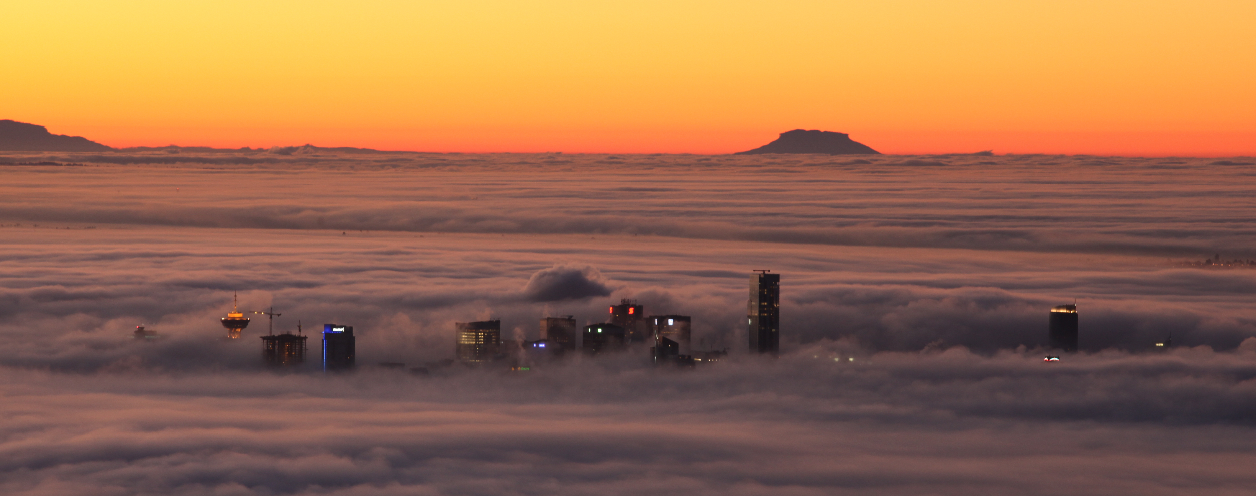
\includegraphics[width=\linewidth]{CypressView}
%  \caption{In the Clouds: Vancouver from Cypress Mountain. Note that the teaser may not be wider than the abstract block.}
%	\label{fig:teaser}
%}

%% Uncomment below to disable the manuscript note
%\renewcommand{\manuscriptnotetxt}{}

%% Copyright space is enabled by default as required by guidelines.
%% It is disabled by the 'review' option or via the following command:
% \nocopyrightspace

\vgtcinsertpkg

%%%%%%%%%%%%%%%%%%%%%%%%%%%%%%%%%%%%%%%%%%%%%%%%%%%%%%%%%%%%%%%%
%%%%%%%%%%%%%%%%%%%%%% START OF THE PAPER %%%%%%%%%%%%%%%%%%%%%%
%%%%%%%%%%%%%%%%%%%%%%%%%%%%%%%%%%%%%%%%%%%%%%%%%%%%%%%%%%%%%%%%%

\begin{document}

%% The ``\maketitle'' command must be the first command after the
%% ``\begin{document}'' command. It prepares and prints the title block.

%% the only exception to this rule is the \firstsection command
\firstsection{Introduction}

\maketitle

%% \section{Introduction} %for journal use above \firstsection{..} instead
%% This template is for papers of VGTC-sponsored conferences such as IEEE VIS, IEEE VR, and ISMAR which are published as special issues of TVCG. The template does not contain the respective dates of the conference/journal issue, these will be entered by IEEE as part of the publication production process. Therefore, \textbf{please leave the copyright statement at the bottom-left of this first page untouched}.

Direct volume rendering (DVR) is a pervasive visualization technique for displaying 3D scalar fields with applications in engineering, material sciences, and medical imaging sciences. However widely adopted, and able to handle large datasets at interactive rates, DVR inherently suffers from the problem of \emph{occlusion}: Structures of interest located deep in the volume, called next \emph{targets}, can be hard to spot and/or explore.

To aid with this, various techniques have been designed including transfer functions, segmentation, selection, and clipping. Yet, all such techniques have limitations.  \emph{Global} mechanisms, like transfer function editing, can remove both occluders and targets if these have similar densities. In certain applications, carefully designed transfer functions exist and should be used without (significant) modifications to facilitate understanding and user training\,\cite{4276082}. \emph{Local} mechanisms like segmentation, selection, or clipping are more effective in manipulating data confined to a given spatial region. Yet, many such mechanisms assume that one can easily and accurately select targets to remove them (occluders) or keep them (occluded). This is hard to do when \emph{e.g.} one does not have direct access to the targets, or when significant 3D interaction is required to select occluder(s).

A different way to handle occlusion is to use \emph{lenses}. These are flexible lightweight tools which enable local and temporary modifications of the DVR to reveal targets while keeping the global visualization context\,\cite{595268,CGF:CGF12871,6327262}. However, efficiently selecting the target and  removing all in-between occluders is still challenging. In detail, most existing occlusion management techniques do not simultaneously meet all following requirements:
Rapidly create an unobstructed view of the target (R1), 
allow an easy change of all parameters (R2), 
keep the global context (R3), 
and handle datasets where the target and occluders have very similar densities (R4).

In this paper, we increase the flexibility of lenses for DVR exploration to jointly cover all above requirements. We propose a focus-and-context (F+C) lens that combines a distortion technique, which pushes aside the occluding objects, with a fish-eye field of view, to provide a better perspective on targets. We specifically target the use-case of \emph{partially occluded} objects, where the user has a glimpse of an interesting structure, buried deep in the data, but only slightly visible from a given viewpoint and transfer-function setting. We allow the user to `open up' the volume without changing these settings, and reveal the target, by simple point, click, and scroll operations. Next, we provide several F+C modifications of the lighting parameters, transfer function, and geometry in the focus area to better understand the target. Our technique, implemented using a CUDA-based approach, can be easily incorporated in any generic DVR system.
 
%ALEX: Removed below text, it's not really related to our contribution here
%Furthermore, performances are still a  challenge in volume rendering systems. In fact, depending on the size of the dataset and also the resolution of the resulting produced image: the rendering process can be very slow. Some optimization strategies such as empty space skipping~\cite{Liu:2009:AVR:2421899.2421919}, early ray termination~\cite{CGF:CGF12605}, multiple and adaptive resolutions allow to speed up the rendering process by increasing the frame rate. With the advent of CUDA as a higher-level GPU programming language, CUDA-based ray-casters were introduced~\cite{Kainz:2009:RCM:1661412.1618498}. 

The paper is structured as follows. Section~\ref{sec:related_work} presents related work in occlusion management, lenses, and deformations for DVR visualization. Section~\ref{sec:principle} introduces the principle of our lens. Section~\ref{sec:implem} introduces implementation details. Section~\ref{sec:scenarios} presents five application scenarios for our lens in baggage inspection, 3D fluid flow visualization, chest radiology, air traffic planning, and DTI fiber exploration. Section~\ref{sec:discussion} discusses our proposal. Finally, Section~\ref{sec:conclusions} concludes the paper.



\section{Related work}
\label{sec:related_work}
%
To start with, let us refine requirements R1$,\ldots,$R4.

\noindent{\textbf{R1:}} The technique should rapidly create an unobstructed view of the target, \emph{i.e.}, such a view should be created at interactive frame rates (10 fps or more) with no special pre-processing of the input volume (\emph{e.g.}, segmentation), and with minimal user input (\emph{e.g.}, using simple mouse and/or keyboard-modifier events). All above are needed to ensure that one can freely \emph{explore} the volume by activating the lens anywhere with minimal effort and seeing its effect in real-time.

\noindent{\textbf{R2:}} Allowing a flexible exploration of the target zone means that one can manipulate the zone in the lens in various ways to see how the target is actually embedded in its surrounding context.

\noindent{\textbf{R3:}} Keeping the context means that the visualization around the lens does not change significantly from what would be shown there if the lens were not activated. This is needed to maintain the user's mental map before \emph{vs} after activating the lens.

\noindent{\textbf{R4:}} The lens should enable the exploration of datasets where targets cannot be easily separated (isolated) from their surrounding context simply by manipulating parameters of the transfer functions (TF). One such issue is when targets and surrounding zones have similar densities; in this case, using a single global opacity TF could either render everything opaque (thus, it will be hard to visually isolate the target) or highly transparent (thus, the zone around the target will be transparent but so will be the target too).

Previous work on handling occlusion when exploring volume data can be divided into occlusion management techniques and lenses-and-deformation techniques. We next discuss these and also point out limitations from the perspective of R1$,\ldots,$R4.

\begin{figure*}[htbp]
\centering
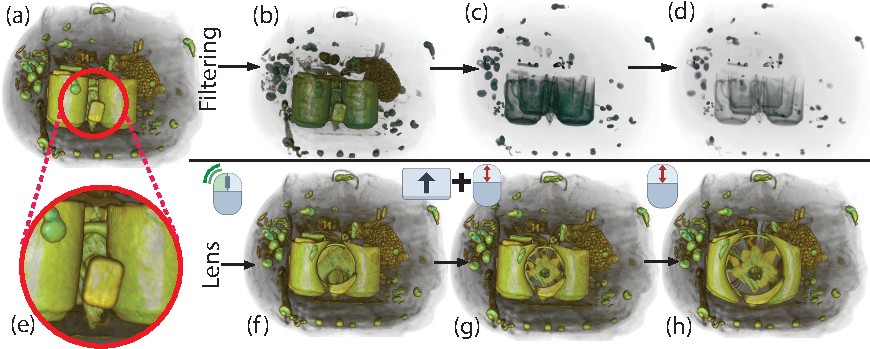
\includegraphics [width=0.9\textwidth]{shuriken.eps}
\vspace{-0.15cm}
\caption{(a-c) A baggage scan is viewed from different angles. In view (c), a suspicious sharp object is spotted between a set of mugs. (d-f) Filtering densities using a classical 1D opacity transfer function removes progressively more of the occluders (mugs), but also the target. (g) The user applies the lens on the target object (double-click). An animation starts opening the lens, rays are gathered to pass through occluders. Halfway through the animation, the object is magnified, but only the area close to the lens is visible. (h) The fish-eye field of view at the end of the animation scatters rays to fully show the target. (i) The lens is increased to magnify the target (mouse scroll).}
\label{f:baggage_lens}
\end{figure*}
\vspace{-0.15cm}


\subsection{Occlusion management}
%
Many occlusion management approaches have been proposed\,\cite{4483791}. Multiple viewports show the data from different perspectives\,\cite{WangBaldonado:2000:GUM:345513.345271}. This does not help when the target is strongly occluded from \emph{all} possible viewpoints (R4). Virtual X-ray methods make targets visible by turning occluders (half-)transparent\,\cite{Burns:2008:ACC:1457515.1409107}. Kruger et al.\,\cite{4015450} proposed ClearView, which interactively focuses on specific areas in the data while preserving context without visual clutter by modulating transparency. Correa and Ma\,\cite{5416704} proposed visibility-driven transfer functions (TFs) to maximize the visibility of selected data-intervals. Designing good TFs is still challenging (R2) in general: For instance, in baggage inspection, a dissimulation strategy is to hide a threat among same-density objects, so TF editing cannot easily remove occluders but keep the target (R4)\,\cite{7819413}. De-occluding a tumor from surrounding similar-density tissue in medical scans is a similar situation\,\cite{CGF:CGF12927}. 
Rezk-Salama and Kolb\,\cite{CGF:CGF979} also considered the voxels' occurrence on the cast ray, besides their densities and positions. Hurter et al.\,\cite{moleview,6787171} removed occluders in 2D images, volumes, and trail-sets by deforming (pushing them away) in a focus area. Occludes are selected based on data value-ranges, thus we have here the same limitation as ClearView (R4). Li et al.\,\cite{Li:2012:LVV:2425296.2425325} proposed luggage virtual unpacking where targets are cleared by interactively moving away occluders. This, however, alters the \emph{context} (relative position, connectivity) where occluders occur (R3). Recently, an interactive volumetric data exploration via direct voxel manipulation was proposed\,\cite{7819413}. Extending such approaches in a DVR setting to more complex deformations or changes of the data-in-focus is computationally challenging (R1).

\vspace{-0.15cm}
\subsection{Lenses and deformations}
%
An interactive lens is a lightweight tool to solve localized visualization problems by temporarily altering a selected part of the visual data representation\,\cite{CGF:CGF12871}, and hence provides focus-and-context (F+C) solutions to volumetric data occlusion (R2). Parametrizable lens properties include position, shape, appearance, size, orientation, and selection of included data (focus). The lens \emph{shape} is usually chosen to meet the requirements of the application and is linked to the lens function. Most lenses are circular\,\cite{1648236} (a design we also choose), rectangular\,\cite{Kincaid:2010:SFA:1907651.1907963}, or adapt their shape to the data-in-focus\,\cite{Pindat:2012:JCA:2380116.2380150,Thiede2008}. The lens \emph{position} and \emph{size} can be changed manually by the user, or automatically to guide users toward interesting events in the data\,\cite{Tominski:2011:ECU:2336207.2336211} or along a path of interesting events\,\cite{Alvina:2014:RER:2598153.2598200}. Our lens updates automatically its properties once a target has been selected. This allows a smooth transition towards an unobstructed and magnified area of interest.

Lenses for DVR face spatial selection and occlusion challenges. Magic Lens\,\cite{1532818} addresses these by rendering occlusions with lower opacity and magnifying pre-computed features interactively or automatically in a pre-segmented dataset. This, however, does not provide an (interactive) way to deal with similar-density occluders and targets (R4) and does not propose local exploration of the target context (R2). GlyphLens\,\cite{7539643} removes occluding glyphs by pulling them aside through animation. However, this covers only glyph-based and not DVR visualizations. 

Lenses can create discontinuities between their inside and outside areas. Deformations can be a solution to this.
Hsu et al.\,\cite{Hsu:2011:RFM:2070781.2024165} create flexible deformations by non-linearly sampled rays to smoothly project objects at multiple levels of detail. However, this is computationally expensive and far from real-time (R1). Exploded views are used to partition a volume into several segments\,\cite{Sonnet:2004:IEA:989863.989871,4015467}. This strongly reduces occlusion but distorts the context (R3) and requires some sort of data pre-segmentation which takes time to compute (R1). Correa et al.\,\cite{Correa:2007:IDD:1313046.1313163,Correa:2006:FAV:1187627.1187827} allow one to manipulate the geometry of a data object. McGuffin et al.\,\cite{1250400} performed deformations using peeling to see hidden parts of the data. Such techniques remove potentially important contextual information surrounding the target, which makes it hard to see how the target is embedded in its context (R2).

Deformations can reveal specific data features by using a precomputed segmentation. Tong et al. proposed a deforming lens which moves streamlines to observe the inner part of streamline bundles\,\cite{7332955}. Other techniques performed deformations using surgical metaphors\,\cite{4069230,Correa:2006:FAV:1187627.1187827} to show hidden parts of a volume. Such techniques do not offer tools for local manipulation of the viewpoint that allows seeing a target under multiple perspectives (R2) while keeping the global context. 

Using non-straight-line rays is another way to avoid occluders. Cui \emph{et al.}\,\cite{cui10} propose curved (B{\'e}zier) rays to support this. Wu \emph{et al.}\,\cite{wu16} refine this further to create multi-perspective views. These approaches require a quite careful ray-path planning in advance, so they are not directly aimed at a lens effect (R2). Also, the target should be accessible from the viewpoint via a (possibly curved) path (R4). Also, from the presented examples, although two examples of DVR models are given, it seems these techniques mainly address de-occlusion in large 3D polygonal scenes such as terrain and city models.

Table~\ref{tab:methods} summarizes the main advantages and limitations of a set of volumetric exploration techniques selected from the ones mentioned above which are close to our proposal. As visible, none of the techniques scores high on all requirements. The table also lists the number of different datasets and/or use-cases these techniques were tested on. We will validate our proposal on a similar number of use-cases (Sec.~\ref{sec:scenarios}).
\begin{table}[htbp]
\centering
\small
\begin{tabular}{ |c|c|c|c|c|c| }
\hline
\textbf{Technique} & \textbf{R1} & \textbf{R2} & \textbf{R3} & \textbf{R4} & \textbf{Use-cases}\\
\hline
\hline
McGuffin \emph{et al.}\,\cite{1250400} & + & -- & + & + & 1\\
Sonnet \emph{et al.}\,\cite{Sonnet:2004:IEA:989863.989871} & +/- & -- & + & +/- & 5\\
Wang \emph{et al.}\,\cite{1532818} & + & -- & + & +/- & 6\\
Bruckner \emph{et al.}\,\cite{4015467} & +/- & -- & -- & + & 6\\
Correa \emph{et al.}\,\cite{Correa:2007:IDD:1313046.1313163,Correa:2006:FAV:1187627.1187827} & + & -- & + & + & 8\\
Cui \emph{et al.}\,\cite{cui10} & + & -- & + & -- & 5\\
Hsu \emph{et al.}\,\cite{Hsu:2011:RFM:2070781.2024165} & -- & +/- & + & + & 4\\
Hurter \emph{et al.}\,\cite{6787171} & + & +/- & + & -- & 6\\
Wu \emph{et al.}\,\cite{wu16} & + & -- & + & -- & 5\\
\hline
\end{tabular}
\caption{Related work selection \emph{vs} requirements R1..R4 ('+': good, '+/-': average, '--': limited) and the number of use-cases (datasets) used to demonstrate these methods.}
\label{tab:methods}
\end{table}



\vspace{-0.09cm}
\subsection{Detailed contributions}
%
Summarizing the above discussion on the requirements and related work on occlusion management, we propose a new technique which combines high-quality DVR with a fast, versatile, and easy to use, lens to support the interactive exploration of occluded data in volumes. In the classification of view deformations by Carpendale \emph{et al.}\,\cite{595268}, we use a nonlinear radial distortion through an interactive lens to remove occluding items and keep the global context while magnifying a partially occluded item. Related to volumetric lens techniques, we frame our contribution as follows: We propose an interactive deforming lens that magnifies and pushes aside occluding objects located in front of a designated focal point which meets the four requirements; the combination of flexible and real-time interactive changing of the focal point, custom bent rays used for DVR, lens deformation, and shading and transfer function in the focus area allow us to provide \emph{on the fly} a range of perspectives of the targets, without having to change the viewpoint or manipulate complex parameters in multiple linked views.



\begin{figure*}[htbp]
\centering
\vspace{-0.15cm}
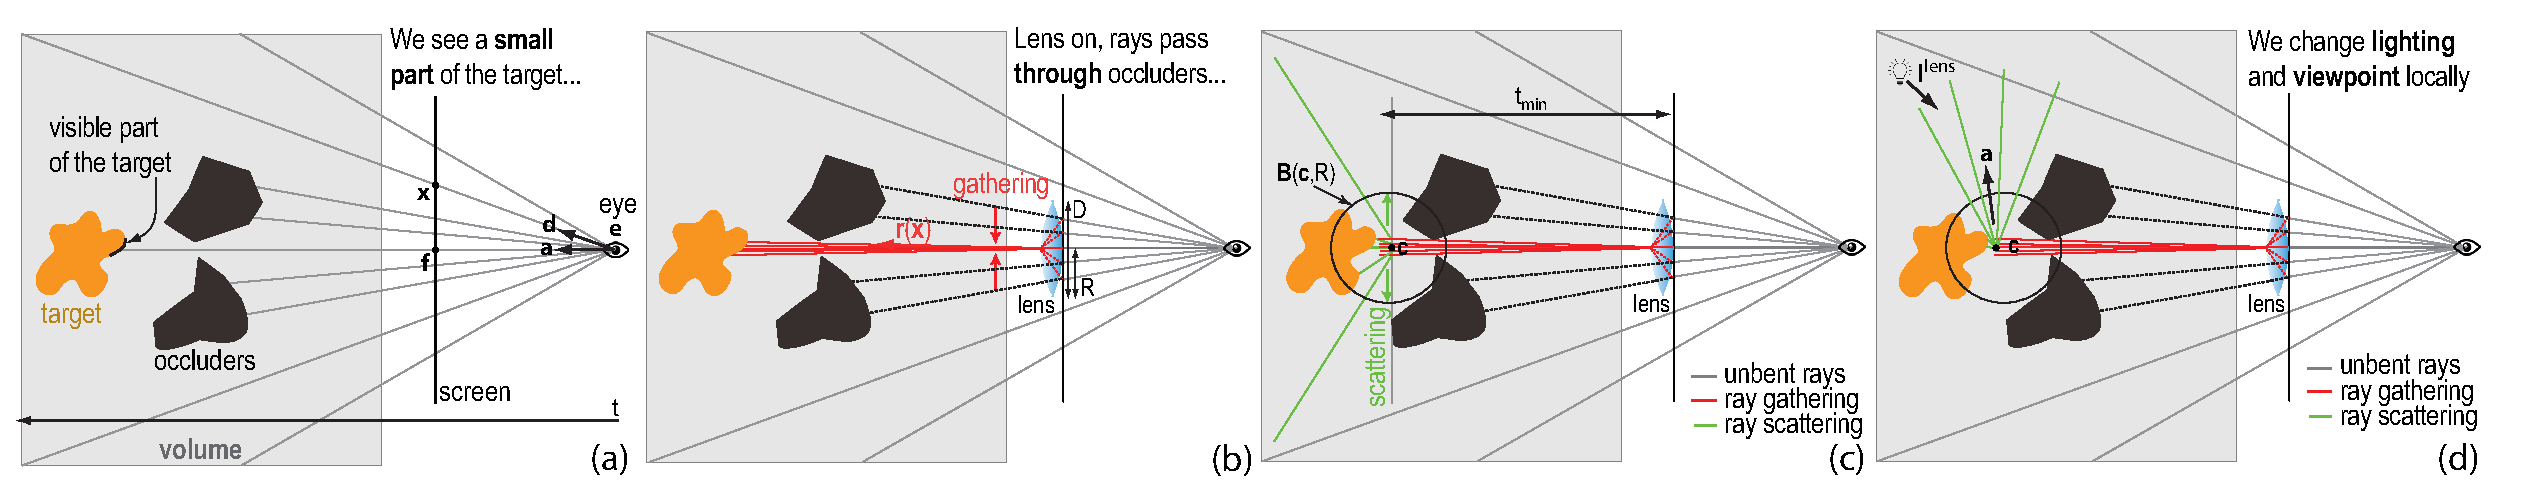
\includegraphics [width=0.99\textwidth]{images/principle.eps}
\vspace{-0.15cm}
\caption{Principle of the obstruction-free lens. An interesting target object is mostly hidden by occluders in front of it. (a) Classic raycasting result shows a small part of the target. (b) Our lens gathers the rays to avoid occluders. Once close to the target, rays follow again their initial paths. However, only a small part of the target is visible. (c) Scattering the rays makes the full target visible.}
\label{f:fisheye}
\vspace{-0.15cm}
\end{figure*}

\vspace{-0.15cm}
\section{Principle}
\label{sec:principle}
%
%
Our proposed lens combines the modification of several parameters of a typical DVR rendering of volume data, as follows. Consider the typical DVR algorithm: Given a scalar volume $V \subset \mathbf{R}^3 \rightarrow \mathbf{R}$, each pixel $\mathbf{x} \in I$ in the DVR image $I \subset \mathbf{R}^2$ thereof corresponds to the compositing of sampled data along a ray starting passing through $V$ and ending at $\mathbf{x}$. In classical DVR (\autoref{f:fisheye}-a), such rays are defined by the eye position $\mathbf{e}$ and a ray direction unit vector $\mathbf{d} = (\mathbf{x} - \mathbf{e}) / \| \mathbf{x} - \mathbf{e} \|$ pointing from $\mathbf{e}$ to $\mathbf{x}$. Consider next a focus point $\mathbf{f} \in I$ (the \emph{lens center}) and a lens radius $R > 0$. In our proposal, we modify all rays traveling through the disk $D = \{\mathbf{x} \in I | \| \mathbf{x} - \mathbf{f} \| \leq R\}$, or \emph{focus area}, in order to de-occlude, magnify, and emphasize a target object. Our new ray behavior can be divided into three steps: (1) Provide an unobstructed view of the occluded object. This moves closer to the target while avoiding the obstacles by pushing them aside. (2) Set a wide field-of-view (fisheye) to better see the target. (3) Interactively modify various parameters of the lens, lighting, and opacity TF in real time to better explore the target. These steps are detailed next.

\vspace{-0.15cm}
\subsection{Creating an unobstructed view}
\label{sec:gathering}
%
The scenario our lens addresses is as follows: Given a volume $V$, users produce a DVR thereof, using whatever suitable TFs and other parameters are applicable. When examining $V$ from various viewpoints, (at least) one viewpoint $(\mathbf{e},\mathbf{d})$ is found from which some intriguing structure is \emph{partially} visible in $I$. We call this structure the \emph{target}. Users next want to quickly and easily unravel the target. For this, we proceed as follows: We first \emph{gather} all rays passing through the lens pixels (focus area $D$) to follow the lens' axis vector $\mathbf{a} = (\mathbf{f} - \mathbf{e}) / \| \mathbf{f} - \mathbf{e} \|$. As explained above, at the location $\mathbf{f}$ of the lens center, we do see an interesting partially occluded target. Hence, by definition, the gathered rays pass \emph{through} occluders to hit this target, otherwise we would not see it. We control gathering by setting the ray direction passing through $\mathbf{x} \in D$ to
%
\begin{equation}
\mathbf{r}(\mathbf{x}) = (1-\alpha) \mathbf{a} + \alpha \mathbf{d},
\label{eqn:gathering}
\end{equation}
%
with $\alpha \in [0,1]$. When $\alpha=0$ (default value), all rays follow the lens axis $\mathbf{a}$, thus, can best pass through obstacles. When $\alpha=1$, rays follow their original classical DVR path. Changing $\alpha$ with the mouse wheel allows one to smoothly navigate between the lens effect, \emph{i.e.} opening up a `hole' in the volume to see the target, and a classical DVR visualizaton of the volume.
%
\vspace{-0.15cm}
\subsection{Setting a wide field of view}
\label{sec:scattering}
%
Once the rays pass obstacles (Sec.~\ref{sec:gathering}), we want to \emph{scatter} them so as to best sample the target. Consider that this target is at some depth $t_{target}>0$ within $V$. After the rays pass the occluders, but before they hit the target, \emph{i.e.}, travel past a distance $t_{min} < t_{target}$ through $V$, we deflect (scatter) them so as to best sample the target. For this, we set the parametric position of a ray point to
%
\begin{equation}
\mathbf{p}(\mathbf{x}, t) = \mathbf{r}(\mathbf{x})t + \beta (\mathbf{x}-\mathbf{f})(t-t_{min})
\label{eqn:scattering}
\end{equation}
%
for any pixel $\mathbf{x} \in D$ and any $t \geq t_{min}$. Here, $\beta \geq 0$ controls the ray scattering: Small values magnify a small volume area located close to the ray $\mathbf{r}(\mathbf{x})$; larger values sample more of the volume area behind the lens. Intuitively, this works as if we moved a maginfying lens to a depth $t_{min}$ inside $V$. Summarizing, after the user finds an interesting but partially occluded target using \emph{standard} DVR, the lens squeezes rays to pass between occluders and next fans them out to reveal the target in full detail. The parameter $\beta$ can be adjusted by the user via the mouse scroll wheel while pressing the Shift key (\autoref{f:fisheye}-c).
%
%

\begin{figure*}[htbp]
\centering
\includegraphics [width=0.97\textwidth]{images/params.eps}
\vspace{-0.15cm}
\caption{Changing lighting parameters in the lens. (a) Constant specular coefficient. (b) High specular coefficient in the lens. (c-f) Changing the in-lens light vector yields the effect of a flashlight rotating around the target.}
\label{f:params}
\vspace{-0.15cm}
\end{figure*}

\vspace{-0.15cm}
\subsection{Interactive exploration of the target}
%
We allow users to interactively modify several parameters of the DVR and the lens to achieve a more effective exploration, as follows.

\vspace{0.2cm}
\noindent\textbf{Lens radius:} The lens radius $R$ can be controlled via the mouse wheel, thereby specifying how big is the `hole' to open up in the volume to see the target. The parameters $\alpha$ and $\beta$ controlling respectively the gathering and scattering of rays are controlled by the mouse wheel and modified keys. The value $t_{min}$ controlling the depth from which scattering starts is controlled using the arrow keys.

\vspace{0.2cm}
\noindent\textbf{Lens axis:} Users can rotate the lens axis $\mathbf{a}$ using a virtual trackball activated by the right mouse button. Changing this direction effectively samples the target from many viewpoints, thereby allowing the user to look `around' it so as to see its parts which are not visible from the current viewpoint, but \emph{without} having to actually change the viewpoint. This is of high added value, since changing the viewpoint may bring us to a view in which the target is completely invisible, so we do not know where precisely to activate the lens any more. Figure~\ref{f:rotation} shows three such local rotations for the baggage dataset introduced in Fig.~\ref{f:baggage_lens}. From these, we see that the star-shaped target is relatively thick.

\begin{figure}[htbp]
\centering
\includegraphics [width=0.48\textwidth]{images/rotation.eps}
\vspace{-0.15cm}
\caption{Performing local rotations in the lens allows better seeing the shape and thickness of the target object.}
\label{f:rotation}
\vspace{-0.15cm}
\end{figure}


\vspace{0.2cm}
\noindent\textbf{Lighting:} We modify the volumetric Phong lighting parameters to better explore the target, as follows. Let $\mathbf{c} = \mathbf{e} + t_{min}\mathbf{a}$ be a point at depth $t_{min}$ along the lens axis, and let $B(\mathbf{c},R)$ be a sphere of radius $R$ around this point (\autoref{f:fisheye}b). We call voxels in this sphere `in focus', and all other voxels in $V$ `out of focus'. Let $\phi$ be the specular term coefficient, set to a high value (default: one).

First, for all voxels $\mathbf{x} \in B(\mathbf{c},R)$, we use a specular coefficient $\phi(\mathbf{x}) = \phi (1-d)$, where $d=\|\mathbf{x}-\mathbf{c}\|/R$. For all voxels outside $B(\mathbf{c},R)$, we use $\phi(\mathbf{x}) = 0$. Hence, voxels close to the focus point $\mathbf{c}$ appear highly specular; further away from $\mathbf{c}$, voxels become less specular, and voxels out of focus appear purely diffuse. Secondly, we allow the user to locally rotate the light vector using the same trackball mechanism as for the lens axis rotation. Let $\mathbf{l}^{lens}$ be this vector, and let $\mathbf{l}^{global}$ be the global light vector used by standard DVR. Secondly, for all voxels in focus, we use a light vector $\mathbf{l}(\mathbf{x}) = (1 - d)\mathbf{l}^{lens} + d\mathbf{l}^{global}$. As the user rotates $\mathbf{l}^{lens}$, the light direction will visibly change in the middle of the lens, stay constant outside it, and smoothly change in between.

The above two mechanisms combined yield the effect of a moving flashlight turning around a shiny target, surrounded by a constantly-lit diffuse scene. This highlights small-scale details on the target surface, again, without having to change the viewpoint or lens location. Additionally, the high specularity in the lens attracts the user's attention to this focus area; the diffuse lighting outside the lens put less emphasis on this context area.

\vspace{0.2cm}
\noindent\textbf{Opacity:} Finally, we modify the opacity transfer function along a similar idea as for lighting. Let $TF_{o}^{global} : \mathbf{R} \rightarrow [0,1]$ be the user-chosen opacity function used globally for the volume. Let $\Gamma$ be a Gaussian pulse of unit height centered at the average density value $\bar{\rho}$ in $B(\mathbf{c},R)$ and with standard deviation $\sigma$. We estimate $\bar{\rho}$ and $\sigma$ by considering the density $\rho$ at 150 points randomly sampled inside $B(\mathbf{c},R)$. Then, for voxels in $B(\mathbf{c},R)$, we use an effective opacity transfer function $TF_o = TF_{o}^{global} + (1-d) \Gamma$. For voxels outside $B$, we use $TF_{o}^{global}$, as in standard DVR. The effect is that voxels in $B$ become ore opaque, thus more visible. Tet, voxels having the same densities but outside $B$ will use the default transfer function, which can make them transparent. This allows to have voxels with similar densities either opaque (if close to the target, thus of interest) or transparent (if they are \emph{e.g.} in front of the target, thus occluding).

\subsection{Smooth transitions}
\label{continuity}
%
If we apply Eqns.~\ref{eqn:gathering} and~\ref{eqn:scattering} to bend rays passing through the lens pixels $D$, and trace all other rays starting at pixels in $I \setminus D$ as straight lines, discontinuities appear at the lens borders. We solve this as follows. Let $\mathbf{p}(\mathbf{x},t)$ be the voxels along a lens ray starting at screen pixel $\mathbf{x}$, as computed by Eqn.~\ref{eqn:scattering}. Let $\mathbf{p}^{line}(\mathbf{x},t)$ be the voxels computed along an straight-line ray starting at the same pixel, \emph{i.e.}, using $\alpha=1$ and $\beta=0$ in Eqns.~\ref{eqn:gathering} and~\ref{eqn:scattering} respectively. For every value $t$ along every such ray, we compute the interpolated ray
$\bar{\mathbf{p}}(\mathbf{x},t) = (1-f(d))\mathbf{p}(\mathbf{x},t) + f(d)\mathbf{p}^{line}(\mathbf{x},t)$, where $d$ is the distance of $\mathbf{x}$ to the lens axis (normalized to unit by dividing it by $R$) and $f : [0,1] \rightarrow [0,1]$ is an interpolation function. Next, we use the rays $\bar{\mathbf{p}}(\mathbf{x},t)$ to compute the DVR by standard composition. This way, rays effectively vary smoothly from their bent versions (close to the lens axis) to straight lines (outside the lens). Setting $f(d) = d^2$ keeps the interpolation transitions close to the lens border, so most of the lens is dedicated to show the desired fisheye effect.

Separately, we use a slow-in/slow-out animation~\cite{Dragicevic:2011:TDA:1978942.1979233} to introduce the lens effect. When the lens is activated, we vary the values of $\alpha$ and $\beta$ from their defaults ($\alpha=1$, $\beta=0$, \emph{i.e.} straight-line classical DVR) to their actual user-set values, compute the volume rendering on-the-fly, and display the resulting images. The overall effect resembles gradually opening a hole in the volume -- see the associated video. The speed increase at the start of the animation helps one to quickly see what is revealed in the lens; the decreasing speed at the end helps seeing where the pushed-away occluders actually go. This also gives some semantic to the moving shapes, allowing the human mind to interpret the motion as a magnification of a target, and to keep the focus on visual entities during this transition. When the lens is deactivated, we play back the animation in the opposite sense, which suggests closing the opened hole in the volume.

\section{Implementation}
\label{sec:implem}
%
We implemented our occlusion-free lens by modifying a standard DVR ray caster implemented in turn using NVIDIA's CUDA platform. Such a ray caster is publicly available in CUDA's SDK\,\cite{cudasdk}. The key changes we applied the definition of the ray (Eqns.~\ref{eqn:gathering} and \ref{eqn:scattering}), and controlling the lens and local per-voxel Phong lighting parameters via mouse and keyboard events. On a PC with 16 GB RAM and a GeForce GTX TITAN X card, we achieve an interactive framerate (15 fps) for volumes up to $512^3$ voxels \textcolor{red}{and a resolution of 1900x1200}. Currently, we use a compositing ray function. However, any other functions can be directly used with no restrictions. All in all, adding our lens to an existing ray caster should pose no significant problems.

\begin{comment}
%ALEX: Commented out the algo pseudocode. There are so far several problems with it, needs to be rewritten, anyways using the current notations. We can see if we have space/time to do it when all else is ready.

Algorithm \ref{alg:propagation} shows a pseudo code of the behavior of our deforming lens

\begin{algorithm}
\SetKwInOut{Input}{Input}
\SetKwInOut{Output}{output}
\SetKwInOut{Parameter}{Parameter}

 \Input{
 $\vec{e}$: the eye position,
 
 $\vec{d}\left(x,y\right)$: the ray direction according to the screen space coordinates of the resulting pixel ($x$ and $y$),
 
 $step$: the sampling distance along the ray.
 
 }
 \KwResult{the pixel color.}
 
 \Parameter{
 $a$: the attraction factor,
 
 $\alpha$: the angle of view.
 }
\BlankLine
 
  $k  \leftarrow $ the normalized distance to the axis of the lens
 $\vec{p}_{near}  \leftarrow \vec{e} + t_{near} \times \vec{d}\left(x,y\right)$ //The initial position  \; 
 $\vec{p}^{0} \leftarrow \vec{p}_{near} $ \; 
 \While{ $ t \le t_{far}$ And $Opacity \le Opacity Threshold  $ }{
 	\If{the current ray is inside the lens}{
    	\If{ $t < t_{target}$ }{
        	$\vec{p}^{1} \leftarrow \vec{p}_{near}\left(x,y\right) + t \times \vec{d}_{target} + a \times \vec{f}_{attraction}$  \;
            \lElse{
        	$\vec{p}^{1} \leftarrow \vec{p}_{target} + \left( t-t_{target} \right) \times \vec{d}_{fishEye}\left( \alpha \right)$
        	}	
        }
               
    $\vec{p} \leftarrow \vec{p}^{0} + f\left(k\right) \times \left( \vec{p}^{1} - \vec{p}^{0} \right) $	\;
     \lElse{
     	 $\vec{p} \leftarrow \vec{p}^{0}$
     }
    }
\emph{Sampling at the position $\vec{p} $ }\;
    
    \emph{Shading the sampled value }\;
    
    \emph{ Compositing the shaded sampling point with the previous values} \;
 
    $t \leftarrow t + step$ \;
    $p^{0} \leftarrow p^{0} + step \times \vec{d}\left(x,y\right)$ \;

}
$color_{final} \leftarrow$ composited colors \;
return $color$
 

\label{alg:propagation}
 \caption{Pseudo code of our lens deformation algorithm}
\end{algorithm}

\end{comment}



\begin{comment}
%ALEX: Already discussed in the appropriate section on streamlines

Moving objects are entities that change locations in space over time. This is the case with aircraft trajectories where an aircraft takes off at a given airport at the beginning of its strip and lands onto another one at the end of its journey. Classical methods use projected lines on a 2D visualization to explore dataset composed of such moving objects \cite{hurter2014interactive}. Even if such methods have shown valuable results, additional insight and data retrieval can be envisaged with other rendering techniques like volume rendering.

\textbf{Dataset rasterization:} While Bresenham's line algorithm is a standard algorithm to turn a line form the vector space to a raster 2D or 3D space, it will not fulfill volume rendering compatibility. Raster line must have a given thickness to maximize the number of intercepting rays and thus ensuring their visualization thanks to volume rendering methods. Other techniques can be envisaged with the computation of meshes (i.e. pipes that encompasses the 3D line) but such computation can create geometric artifacts and might be long to process. Therefore, we used an extended version of the kernel density estimation algorithm \cite{ silverman1986density} into a 3D space. Such method has already shown interesting results with visual simplification and trajectory aggregation \cite{hurter2012graph} and is part of so-called pixel-based visualization \cite{hurter2015image}.
Such process works as follows: we first define a 3D Gaussian kernel of a radius R; the center of this kernel has the highest value, while its border the lowest. Second, we re-sample every trajectory with a minimum distance between two consecutive points inferior to the half of the kernel radius. Third, we compute the convolution of this 3D kernel with the re-sampled trajectories.

Convolution can take time with a large dataset to process, therefore, we turned this computation into the frequential space. Such technique has already been applied with trajectory dataset and can even be accelerated thanks to GPU techniques \cite{lhuillier2017ffteb}.

\end{comment}


\section{Application Scenarios}
\label{sec:scenarios}
%
We next demonstrate our obstruction-free lens via five use-cases considering scalar density volumes from baggage inspection, 3D flow simulation, radiology, air traffic planning, and diffusion tensor imaging.

\subsection{Baggage inspection: An unusual blunt object}
\label{sec:baggage}
%
In airports, security agents deal with volumetric data exploration during baggage inspections. While automatic systems can detect densities of harmful substances such as C-4, TNT, and nitroglycerin, or prohibited articles (threats) like classical firearms and knives, unusual threats are hard to find. Four main concealment strategies exist\,\cite{7819413}:

\vspace{0.15cm}
\noindent\textbf{Superposition}: A threat may be sheltered among dense materials. While possible to see through such a `shield' using high penetration (enhanced X-ray power) or image processing (contrast improvement), such techniques are not universally available and also require fine-tuning many parameters, which slows down inspection.

\vspace{0.15cm}
\noindent\textbf{Location}: Objects located in the corners, edges, or in the luggage's frame are very hard to spot.

\vspace{0.15cm}
\noindent\textbf{Dissociation}: One can conceal a threat by spreading its parts in the luggage, \emph{e.g}, by disassembling a weapon and scattering its parts.

\vspace{0.15cm}
\noindent\textbf{Lure}: A minor threat (lure) like small scissors is clearly visible and catch the security agent's attention who can miss the real threat.

Baggage labeled as suspicious by human inspection or automated scan heuristics must be checked by human agents. Besides time-consuming physical unpacking, one can use `virtual unpacking' tools that segment the 3D scan by a density-based confidence measure and next move the segmented objects away by animation to reduce occlusion\,\cite{Li:2012:LVV:2425296.2425325}. Such systems have been patented and used in production\,\cite{patent}. However, when the automatic segmentation is not optimal, the user must manually change its parameters, repeat the segmentation and animation, which goes back to being time-consuming.

Consider the baggage scan in \autoref{f:baggage_lens} ($283 \times 189 \times 344$ voxels, dataset obtained from an actual airport scan). Automatic baggage inspection systems will not detect anything suspect here. However, while visually exploring this baggage from different angles (\autoref{f:baggage_lens}a-c), we see an object hidden between a set of mugs. To reduce occlusion, a common solution in baggage inspection is to filter materials by density in order to show or hide subsets of the volume. However, for our dataset, the suspect target has almost the same density as the surrounding mugs, so removing the latter also removes the target (\autoref{f:baggage_lens}d-f). Using the obstruction-free fish-eye lens helps here: Clicking on the sharp detail visible in \autoref{f:baggage_lens}c first gathers rays so they pass through the low-density zone between the mugs (\autoref{f:baggage_lens}f). The animation that opens the lens 
(\autoref{f:baggage_lens}e-g) reveals an unobstructed view of the target. However, this shows only a small part of the target. Scattering rays next fully reveals the target (\autoref{f:baggage_lens}h). Adjusting the lens size shows a more detailed view of the target (\autoref{f:baggage_lens}i). Next, locally turning the viewpoint around the target (\autoref{f:rotation}) allows the agent to decide that the target is a shuriken (Japanese ninja star weapon). Since the object is very thick and blunt (see \autoref{f:rotation}), it is not an actual weapon, thus not a threat.

We evaluated our lens for this use-case by a user study. Eight airport security specialists were recruited (ages 23 to 43; experience in baggage scanning 8 months to 20 years, average familiarity with 3D tools from no experience to expert, see Fig.~\ref{fig:questanswers}).
All attended a 20-minute global demo of the lens operation. Next, they were given each a personal training session for using the tool (5 minutes), in which they were instructed on the mouse and keyboard controls. After this, they were asked to work in pairs to examine the above-mentioned baggage CT dataset to form a decision on the nature of the ninja star possible threat (20 minutes of tool usage per person, after which the pair was changed). The idea behind this is that one person operates the tool while the other poses questions or suggest explorations, much like typical airport security operators work with a scanner. In the end, they all separately filled in a web questionnaire covering several questions and also provided open feedback (questionnaire available in the supplementary material). 

Figure.~\ref{fig:questanswers} shows the answers. The first question-set (S1) regarded how easy-to-use, generally effective, and effective \emph{vs} other known tools our lens is for \emph{untargeted} inspection, \emph{i.e.}, when no suspect target is partially visible. Here and next, other tools denote classical 2D X-ray or 3D CT scans used in baggage scanning that the subjects know. As Fig.~\ref{fig:questanswers}c-e shows, 
the answers (on a 5-point Likert scale) were predominantly positive: The tool is easy to use, is useful, and is actually more useful than known tools for untargeted exploration. The second question-set (S2) regarded how good our tool is to examine \emph{specific} targets which are partially visible. Here again, the answers were predominantly positive (Fig.~\ref{fig:questanswers}f-h). The main appreciated features of our tool are listed in Fig.~\ref{fig:questanswers}i.


\begin{figure}[htbp!]
\centering
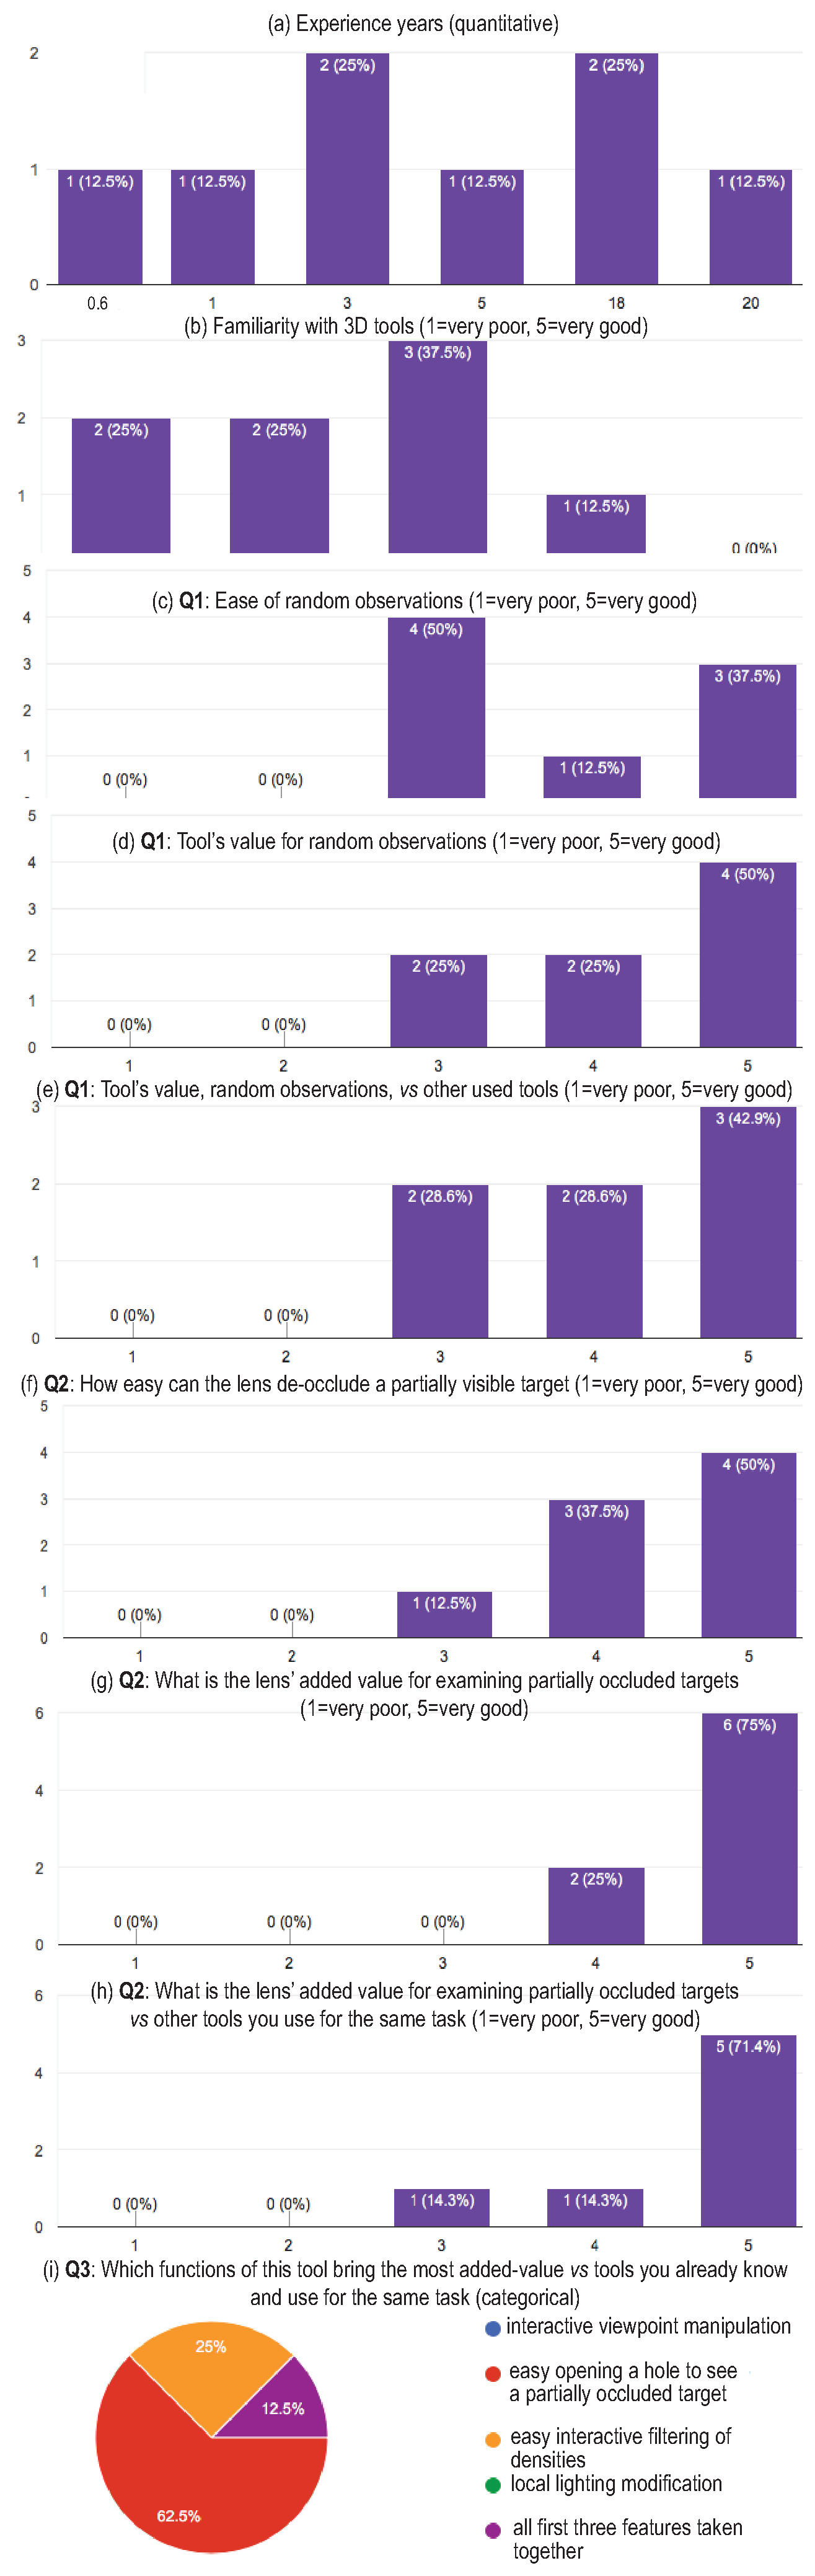
\includegraphics [width=0.42\textwidth]{images/questanswers.eps}
\vspace{-0.15cm}
\caption{Evaluation of lens-based baggage inspection (Sec.~\ref{sec:baggage}).}
\vspace{-0.15cm}
\label{fig:questanswers}
\end{figure}

We next summarize the received open feedback. According to the subjects, our tool can provide them a better perception of the items inside the baggage as compared to the classical 2D single-viewpoint X-ray machinery they routinely use. Quotes from the open feedback: ``clear added-value compared to all systems I know''; ``this tool is a real gain for examining luggage with uniform and/or high densities''; ``definitely better than known tools for examining threats I am not familiar with / I have not seen before''. However, our tool should not be used for the typical carry-on baggage inspection which has a very small allowed inspection time (15 to 20 seconds). Our tool is much more interesting for inspecting checked-in baggage, where inspection time-windows are up to 3 minutes. The perceived added value for this use-case is also higher: Opening up checked-in baggage for manual inspection is much more complicated and time-consuming than for carry-on baggage. Moreover, the only system for inspecting checked-in baggage that the subjects knew of is a scanner that aims to \emph{automatically} detect threats via X-ray imagery; this system suffers from false positives, so a manual examination tool like ours could quickly eliminate such false positives, and thus the delays of opening up checked-in baggage. Finally, several subjects suggested that adding a function to display a classical 2D slice view (activated by a key press and aligned with the focal point) would be useful since this would show additional detail.


\subsection{Fluid flow: A deep-buried spherical vortex}
\label{sec:flow}
%
%
Flow visualization using streamlines has a long history\,\cite{brambilla2012illustrative,merzkirch2012flow}. For 3D datasets, a key challenge is to balance the streamline density. Low values allow seeing inner regions in the data but can subsample (miss) patterns. High values show more data but create too much occlusion. We next show how our lens can be used to alleviate problems in the latter case. The dataset\,\cite{griebel2004flow} captures the simulation of water flow in a basin computed on a grid of $128 \times 85 \times 42$ cells using 4595 streamlines with 183K sample points traced by pseudo-random seeding. We convert this set of 3D curves (polylines) to a scalar volume by using GPU-accelerated kernel density estimation (KDE)\,\cite{lhuillier2017ffteb}. Similar techniques have been used to compute density maps of 2D trail-sets\,\cite{hurter2012graph,cubu,hurter2015image}. 

We first explore the density volume ($500^3$ voxels) using standard DVR (\autoref{f:stream_lens}). Note that, given KDE's smoothing effect, streamlines appear as finite-thickness tubes rather than pixel-thin curves. After turning the viewpoint a bit, we notice a dense spherical item deep in the data (\autoref{f:stream_lens}a). To see its shape better, we increase opacity; however, this immediately increases occlusion so the item becomes invisible. Conversely, decreasing opacity to reduce occlusion makes the item almost transparent. Our lens solves the problem: In the initial view (\autoref{f:stream_lens}a), we point at the target and turn on the lens. This pushes away the occluding stream bundles, and shows that our item is a set of densely-packed, low-speed, tightly-turning streamlines that create a ball-like vortex (\autoref{f:stream_lens}b). 
To make sure our target is spherical, we view it in the lens from different directions, by interactively changing the ray directions in the lens (\autoref{f:stream_lens}c). Finally, we can close the lens but keep the target magnified (\autoref{f:stream_lens}d).
Finding the details of this vortex cannot be done using standard DVR. Interestingly, this vortex has also not been discovered by any of the visualization techniques that used this dataset (according to our knowledge) \,\cite{telea_vis_99,griebel2004flow,ddh,lhuillier2017ffteb}. 

\begin{figure*}[htb]
\centering
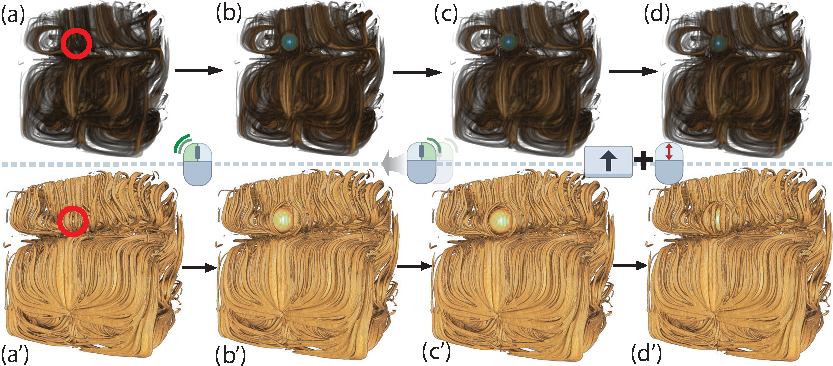
\includegraphics [width=0.95\textwidth]{images/stream_lens.eps}
\vspace{-0.15cm}
\caption{Flow volume exploration with two different opacity transfer functions (top and bottom rows). In viewpoint (a), we notice a small high-density spherical item. (b) We apply the lens at that location (double click). (c) The directions of rays in the lens are changed to see the whole target in the lens (right click + mouse drag change direction). (d) The lens is gradually closed while keeping the focus area magnified (shift + scroll).}
\vspace{-0.15cm}
\label{f:stream_lens}
\end{figure*}

\subsection{Chest scan: A hard to see tumor}
\label{sec:chest}
%
In our third use-case, we consider a contrast chest CT scan ($512 \times 512 \times 110$ voxels) of an elderly patient with a sizeable lung tumor. The tumor was detected in a CT scan performed after the patient reported acute chest pain. Typical examination of these scans by the pulmonologist and radiologist in charge involves slice-based views. Figures~\ref{f:slicer}a-c and \ref{f:slicer}d-f show two such slice sets (axial, coronal, and sagittal views), produced using typical lung, respectively mediastinal, contrast presets. Although the tumor is visible in all these views, its exact shape, morphology, and connection to the lung walls are hard to assess. Finding such details on the tumor is essential, explained the doctors in charge, to determine the TNM score\,\cite{brierley} and also plan treatment. Using standard DVR makes the tumor and its 3D position partially visible (\autoref{f:slicer}f). Yet, occlusion from the rib cage and other tissues is still present. Using both TF presets and manually changing the TFs in the 3D Slicer tool\,\cite{slicer} used to create the DVR could not help de-occluding the tumor without making it partly transparent. The slice images in \autoref{f:slicer}a-f confirm this by showing that the gray values for the tumor and surrounding skin-and-muscle tissue are very similar. This is due to the fact that the tumor had grown rapidly and started necrotizing, which filled it with fluids, making its density very similar to that of the obstructing (skin and muscle) tissue, explained the pulmonologist. Hence, one cannot remove such occluding tissue in a classical DVR setting by opacity TF manipulation without also removing the tumor. This makes examining this specific tumor harder than for regular cases.

\begin{figure}[htb]
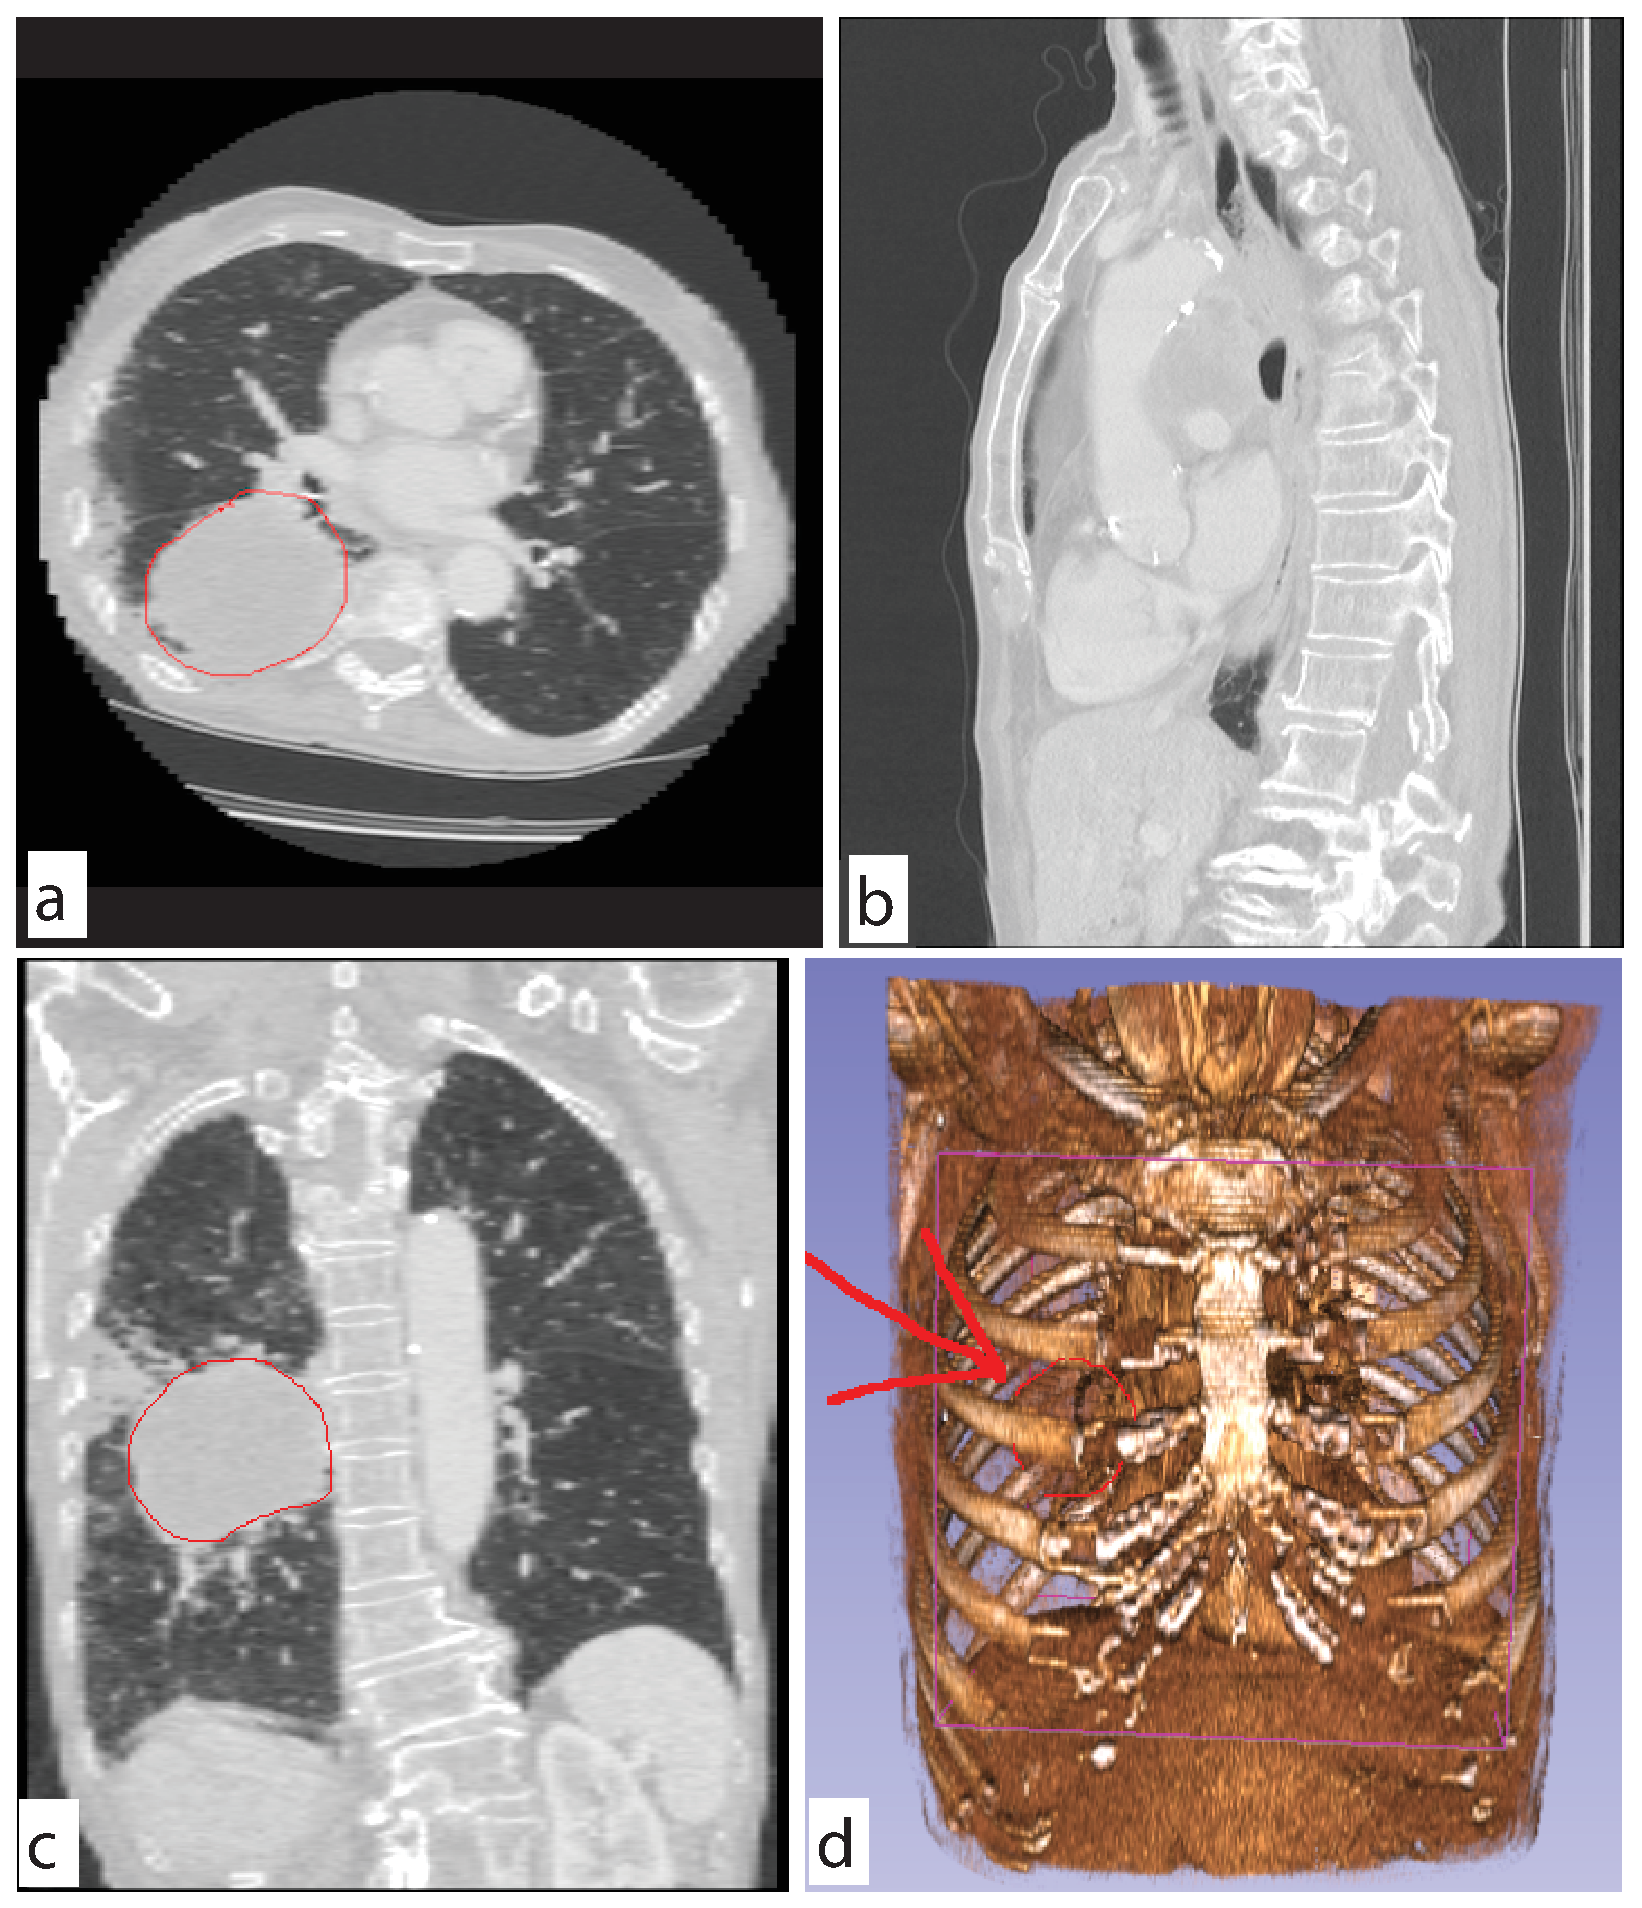
\includegraphics [width=0.48\textwidth]{images/slicer.eps}
\caption{Lung tumor visualization using slices (a-c) and standard DVR (d). Annotations are manually added by the examiner to delineate the tumor location. Images constructed using the 3D Slicer tool\,\cite{slicer}.}
\label{f:slicer}
\end{figure}

We next used our lens to examine the tumor. \autoref{f:params} shows several sample snapshots. We see that the tumor is significantly more visible when using the lens than when using standard DVR (\autoref{f:slicer}d), both in terms of removing the occluding tissue and in terms of the tumor's opacity -- compare the inset in \autoref{f:slicer}d with the images in \autoref{f:params}. Secondly, relighting the tumor from various directions allows one to see small-scale morphological details such as the tumor's surface shape and its connection via protuberances and veins with the lung walls.

We asked the two medical specialists (pulmonologist and radiologist) in charge to state the potential advantages and/or limitations of our lens as compared to standard slicing and DVR techniques, after a 20-minute usage of the tool. 
Both specialists have over 10 years of medical experience in treating lung cancer, and routinely use several slicing and DVR tools. They work in a private hospital in Belgium and are not actively associated with medical imaging research. Our identities were hidden from them during the lens evaluation. The provided input can be summarized as follows: The occlusion-free lens is definitely easier and faster to use than classical DVR and/or slicing techniques. It is especially more effective than these to get a quick, first impression of a deep buried anatomical detail. Changing the lens' parameters by direct interaction is as simple as changing window/level functions in a typical slice-based tool, and is definitely simpler than tuning typical DVR parameters to obtain similar results. This `entices' the user to explore, which is a good aspect. The fact that the lens minimizes viewpoint change (volume rotation), \emph{i.e.}, after a suitable viewpoint was found from which a (small) part of the target is visible, one doesn't need to change this viewpoint, is a strong feature, as 3D viewpoint changes are disruptive and cost time. This is important in a cost-aware environment where specialists have very limited time (about 20 minutes) to assess a CT scan. However, the lens should not \emph{replace} classical slice-based exploration, which shows small-scale details better. In the context of the current dataset (Fig.~\ref{f:slicer}), the lens was useful to both confirm the TNM score (T3 grade tumor, 6.5 cm in size) found via the 2D slices, but much more so for understanding how and where the tumor is connected to surrounding tissue, which is very hard to do using only 2D slices.

\begin{figure}
\centering
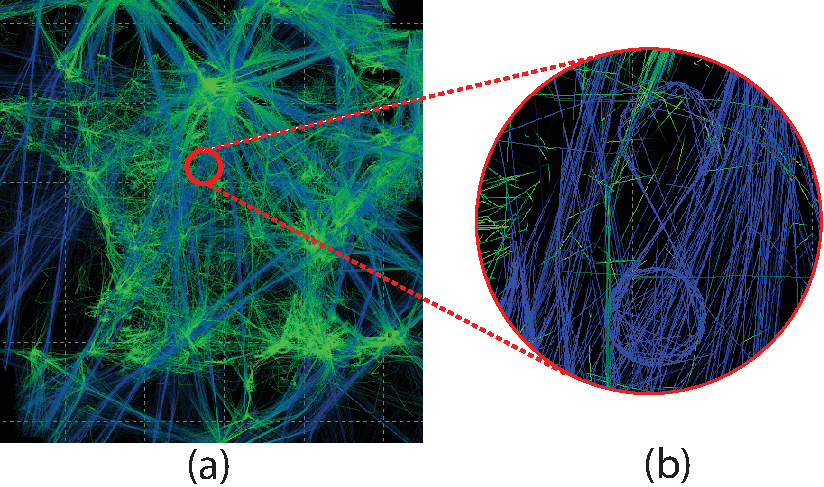
\includegraphics [width=0.48\textwidth]{images/aircraft.pdf}
\vspace{-0.15cm}
\caption{Visualizing one day of aircraft trajectories over France\,\cite{hurter2009fromdady}. (a) Overview of all trails. (b) Zoom, filtering, and color mapping techniques are used to highlight an outlier trajectory of an aircraft performing an eight-shaped loop. Revealing this outlier costs significant user effort.}
\label{f:fromdady}
\vspace{-0.15cm}
\end{figure}


\subsection{Aircraft trajectories: Outliers in the French sky}
\label{sec:atc}
%
%
We next consider a task from air traffic planning -- detecting and studying outliers in large-scale datasets containing tens of thousands of 3D (latitude, longitude, height) trails of aircraft over a given spatio-temporal region\,\cite{hurter2014interactive}. Such datasets are typically viewed using 2D (latitude, longitude) plots where opacity encodes the spatial density of flights -- see \autoref{f:fromdady}a, which shows one day of recorded aircraft trajectories over the French airspace. \autoref{f:fromdady}(b) shows a detail zoom-in, where we can see an abnormal -- that is, far from straight or slightly curved -- aircraft trail: A tanker aircraft performed an eight-shaped loop as it was waiting to refuel other aircraft. Revealing such patterns using 2D techniques, \emph{e.g.} \cite{hurter2009fromdady}, is very hard. In particular, it is hard to de-occlude these patterns from the overall context of criss-crossing aircraft trails, even when one knows their 2D spatial location.

Our lens can help with this task, as follows. We first convert the set of 3D trails to a $500^3$ density volume, using KDE as for the streamline use-case (Sec.~\ref{sec:flow}). Examining this volume via standard DVR shows an outlier trail at some point in space, see curved patterns in \autoref{f:aircraft_lens}a. Activating the lens on this area and interactively tuning the target depth $t_{min}$ (since we don't know the trail's height) beings the outlier trajectory in focus and pushes away occluding trails (\autoref{f:aircraft_lens}a). Like in the other examples presented so far, we can quickly change the magnification factor and view direction to better study this trail in context (\autoref{f:aircraft_lens}b-d). From these images, we easily see that the outlier trail has an eight shape. Revealing this outlier trail using standard 2D visualization techniques\,\cite{hurter2009fromdady} costs several minutes. Doing the same using our lens costs under one minute. Also, comparing Figs.~\ref{f:fromdady}b and~\ref{f:aircraft_lens}b-d, we argue that the eight-shape of the outlier trail is much more prominent, and thus recognizable, in the latter images (made using our lens) than in the former ones. Last but not least, the 3D DVR approach that our lens enhances explicitly encodes flight height information, so our lens can use it by interactively tuning the depth value $t_{min}$ where the lens is focused. This cannot be done with 2D techniques which ignore the depth dimension.

We validated our findings with an air traffic data scientist with more than 10 years of experience in air traffic control and planning. She confirmed that this specific eight-shape trail in \autoref{f:fromdady}(b) is an actual aircraft which performed waiting loops and acted as a fuel supplier for military aircraft. Other comments included the following: Compared to standard 2D visualization techniques, our tool makes detecting outliers easy since there is no need for complex manipulation to reveal such outlier trails. Also, the user does not have to deal with color and alpha mapping parameter-tuning to make specific outliers emerge. Separately, trail visualization easily creates many occlusions leading to either fully opaque areas or too much local overlap, which both hinder seeing and examining specific trails. Our lens does help such cases by distorting the space to locally remove such occlusions. All in all, in the studied dataset (\autoref{f:fromdady}), the lens was specifically useful since, for high transparency, one would not detect the outlier trail, while for low transparency, one would get a hint of the outlier's existence, but not see it in detail due to too much occlusion; the lens allows using low transparency, but removes the clutter caused by it to reveal the outlier.


\begin{figure*}[htbp]
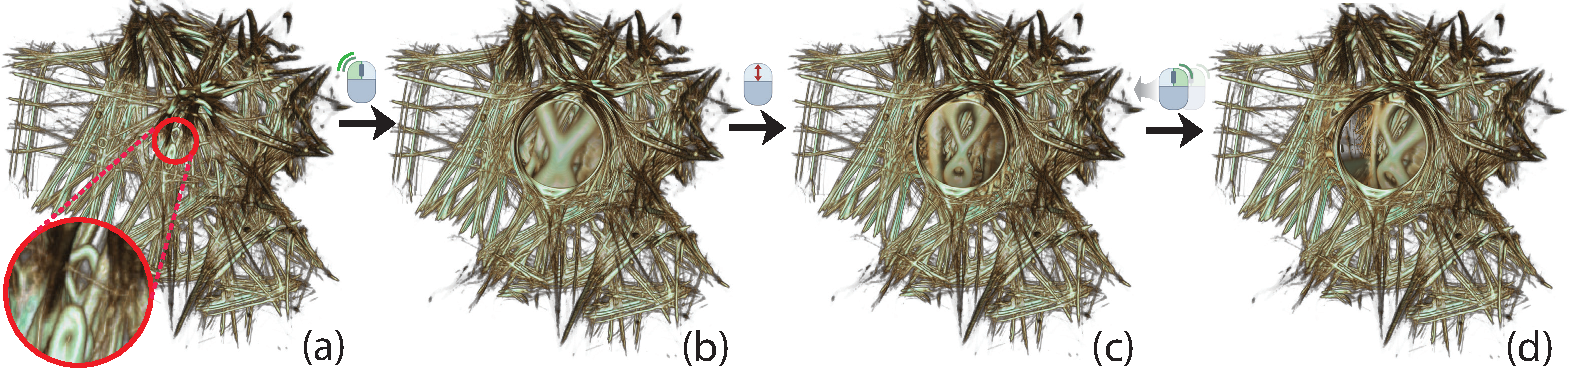
\includegraphics [width=0.98\textwidth]{images/aircraft_lens.pdf}
\caption{Inspecting an abnormal aircraft trail. (a) The abnormal trail is spotted in an all-trails view as it is highly curved while all other trails are relatively straight. Activating the lens at the outlier location (b) and changing the magnification factor (c) reveals the trail's eight-shape. (d) Rotating the viewpoint provides spatial insight on the embedding of the outlier in the surrounding trails.}
\label{f:aircraft_lens}
\end{figure*}
%

\subsection{Brain fibers: Uncluttering the bridge}
\label{sec:dti}
%
Our last use-case considers the exploration of fiber tracts visualized as streamlines of the major eigenvector of a diffusion tensor imaging (DTI) field. Such datasets have a spatially complex structure which makes them hard to explore\,\cite{assaf08}. In particular, fiber tracts are spread volumetrically over the entire extent of the brain, and create tangled patterns inside which it is hard to see much. DVR techniques are often used to render such tracts, one of the advantages being that close fibers get visually `merged' to reveal spatially coherent structures, an effect which is not possible when fibers are rendered as polylines. However, DVR methods also create more occlusion, thus difficulties in seeing structures deep within the volume.

We consider an $128 \times 128 \times 51$ DTI volume (same dataset as in\,\cite{everts15}). We traced 150352 fibers seeded in, and going over, regions of high fractional anisotropy in this volume. We filtered out fibers shorter than 2mm, yielding a total of 120593 fibers to display (6.4M sample points). Next, we converted this fiber-set to a $512^3$ density volume, using KDE with a 3D isotropic kernel of radius 15 voxels, like for the streamline use-case (Sec.~\ref{sec:flow}). Figure~\ref{fig:dti}a shows the result, rendered with DVR, with opacity function mapping the fiber density. While terminal fibers are well visible, we cannot see anything inside the volume. Activating the lens in the middle of the volume opens a hole through which a small part of the \emph{corpus callosum}, the fiber bundle wrapping the bridge that connects the two hemispheres, becomes visible. By slightly decreasing opacity (Fig.~\ref{fig:dti}c), the \emph{corpus callosum} gets clearly visible, appearing as a compact structure, due to the KDE blending of neighbor fibers. Obtaining such a view of the \emph{corpus callosum} only using DVR would be very hard, since transfer functions would either render separated (non-merged) fibers, or else make the fibers surrounding the structure of interest too thick and occluding. 

This scenario has the main difference compared to all previous ones. In all earlier cases, the standard DVR of the data (that is, without the lens) showed us a partial small cue of the structure of interest within the volume, and we used the screen-space location of this structure as the focus point where to activate the lens. In this last scenario, there is no point in the original DVR image (Fig.~\ref{fig:dti}a) from which the \emph{corpus callosum} is even partially visible, due to the high opacity given by the used transfer function. Hence, the user can activate the lens at \emph{any} desired point to peek inside, and towards the center of, the volume. Given the nature of the data, the structure of interest is quite easily visible from most such viewpoints (see lens inset in Fig.~\ref{fig:dti}b). Once its presence is revealed, the user can next adjust the viewpoint and/or the opacity transfer function to get an optimal view on the target, such as the one shown in Fig.~\ref{fig:dti}c. Summarizing, we can use our lens also in cases when no partial view of a target is available. 

\begin{figure}[htb]
\centering
\includegraphics [width=0.40\textwidth]{images/dti.eps}
\caption{Revealing the \emph{corpus callosum} in a DVR of a set of DTI tracts. (a) The \emph{corpus callosum} is not even partially visible in the original DVR image. (b) The structure of interest is quite easily visible from most such viewpoints. (c) The viewpoint and/or the opacity transfer function can be adjusted to get an optimal view on the target.}
\label{fig:dti}
\end{figure}


%

\section{Discussion}
In this paper, we presented four different scenarios where we showed how our lens is a fast and flexible way to overcome occlusion issues: the exploration of a heterogeneous data-set (baggage inspection), the analysis of a deep-buried spherical vortex (fluid flow), the visualization of a hard-to-see lung tumor , and the exploration of a special aircraft trajectory.    

Nevertheless, some aspects of the lens we presented throughout this document suffers from some limitations which we detail in the following. 


First, keeping the continuity between the inner part of the lens and the rest of the volume is very important to preserve a good understanding of object deformations. This is related to the third requirement(R3) which is to keep the global context. To ensure this continuity, we used a linear interpolation function between the final ray trajectory and the one before the previous steps. In fact, the closer a ray is to the lens border, the closer is new trajectory will be to the previous one. We used linear interpolation, whose parameter was modified with a function $ f\left(k\right) = k^2$ in the purpose of reducing the interpolation near the center of the lens. Different functions and mathematical tools could have been used but the result obtained with the current function was satisfying. 

Second, we used a circular lens throughout this study. The circular shape seemed more natural for us but, we could have proposed different lens shapes. At this stage, only the radius can be increased or reduced in order to customize this shape. Furthermore, during the deformation of the rays, the shape of the items considered as obstacles and pushed aside, are modified. It would be interesting to keep their original shapes to improve this focus + context lens (R3). A solution is to adapt our rays' trajectories modification to physical based deformation inside the lens. However keeping the original shapes of all the objects that have been pushed aside can change the global context. In fact, they will either create more occlusion outside the lens or change the items' locations outside the lens by moving them away.  


Third, the angle of view in the second step of our algorithm which allows having a good sight of the targeted item and its local context can be improved. In fact, using a segmentation algorithm that computes the bounding box of the target will help to define precisely and automatically the most suitable angle of view. This is related to the first requirement(R1) which consists in giving a fast unobstructed view on the target. However, we do think it is still important to offer the possibility to modify this angle at will. In fact, this flexibility (R2) allows further exploration of the local context.

Finally, during the first main step of our lens algorithm, we try to get closer to the targeted item or area while pushing the encountered obstacles aside. Automatically finding the right distance to the target, that offers the optimum balance between a good perspective on the full target and obstacle avoidance can be sometimes difficult according to the structure of the data-set (R1 and R4). In our future works, we will instigate automatic curved rays in deforming lens in the purposes of providing in most cases a very good perspective on the target while avoiding occlusion. 

\section{Conclusions}
\label{sec:conclusions}
%
In this paper, we presented a new fish-eye-like context-and-focus lens that addresses the occlusion problems inherent in scalar volume rendering. The principle of our lens consists in first gathering (squeezing) rays so that they easily pass through occluding densities (given a user-specified opacity transfer function) and next scattering (fanning out) rays to best sample the target of interest. Our lens can be directly applied to any DVR raycaster and scalar volume dataset. Its main constraint is that the user should be able to find a viewpoint from which the target of interest, deep buried in the data, is at least slightly visible. We also present several modifications of the local rendering parameters within the lens (view direction, lighting parameters, opacity transfer function) that aim to both better separate the focus (lens) from the context (volume) and also allow more detailed examining of the target. Our lens is easy to use -- all its parameters are controlled via direct mouse-and-keyboard interaction -- and can be efficiently implemented atop of a standard GPU ray caster. Our lens is especially useful for highlighting structures of interest which are both deeply embedded in volumetric data and cannot be revealed by standard transfer function manipulations due to similar densities in the occluders and target. We demonstrate these points using five use-cases involving datasets from baggage detection, fluid visualization, air traffic control, and chest radiology, and DTI fiber tracts.

Several improvements to our proposal are possible, as follows. First and foremost, heuristics can be sought to link all our free parameters (lens size, focus depth, interpolation between focus and context) directly to the volume data, so the user interaction is minimized and therefore exploration efficiency is increased. Secondly, our lens could be extended to different types of volumetric datasets, such as multivariate (vector, tensor) fields. Last but not least, a formal wider-scale evaluation of how the lens addresses more specific tasks, and how it compares to existing tools for these tasks, such as other lens types, is a goal we aim to pursue next.

\section*{Acknowledgments}

The authors acknowledge the support of the French National Agency for Research (Agence Nationale de la Recherche ANR) under the grant ANR-14-CE24-0006-01 project ”TERANOVA” and the SESAR Research and Innovation Action Horizon 2020 under project ”MOTO” (The embodied reMOte TOwer).




%\bibliographystyle{abbrv}
\bibliographystyle{abbrv-doi}
%\bibliographystyle{abbrv-doi-narrow}
%\bibliographystyle{abbrv-doi-hyperref}
%\bibliographystyle{abbrv-doi-hyperref-narrow}

\newpage
\bibliography{template}
\end{document}

